\section{Introducción}\label{introducciuxf3n}

El aprendizaje profundo o Deep Learning comprende una clase de técnicas
englobadas dentro del aprendizaje automático. Esta sección introduce los
conceptos básicos de aprendizaje automático, que son comunes a todas las
técnicas desarrolladas en el ámbito.

Un \emph{algoritmo de aprendizaje}, según \textcite{mitchell1997} es un
programa cuyo rendimiento respecto de un conjunto de tareas \(T\) y una
medida de rendimiento \(P\) mejora tras conocer una experiencia \(E\).
En ese caso, se dice que el algoritmo ha \emph{aprendido} de dicha
experiencia.

Estas tareas y experiencias pueden ser de muy diversas clases, lo que
propicia la aparición de algoritmos y técnicas de aprendizaje diferentes
que tratan de abordarlas. Estos algoritmos computacionales son
necesarios cuando la complejidad o el tamaño de la tarea impide tratarla
con técnicas manuales.

Entre las tareas de aprendizaje que se presentan en la literatura se
incluyen:

\begin{itemize}
\tightlist
\item
  clasificación
\item
  regresión
\item
  detección de anomalías
\item
  agrupamiento (\emph{clustering})
\item
  reducción de dimensionalidad
\item
  detección y eliminación de ruido
\item
  traducción automática
\end{itemize}

Por otro lado, la mayoría de \emph{experiencias} de las que puede
aprender un algoritmo permite categorizarlos en dos grandes clases:
supervisados y no supervisados.

\section{Aprendizaje supervisado}\label{aprendizaje-supervisado}

En este tipo de aprendizaje, se le proporciona al algoritmo un conjunto
de ejemplos para los cuales la tarea está resuelta. Así, se pretende que
aprenda a realizar la misma tarea para nuevos ejemplos.

Un caso particular de esta clase de aprendizaje lo forman los problemas
de clasificación. En ellos, el programa debe deducir para cada ejemplo
una etiqueta o clase, y para ello el aprendizaje se suele realizar
mediante un conjunto de ejemplos que ya tienen asignada su etiqueta.

Entre las aplicaciones del aprendizaje supervisado se encuentran la
clasificación de mensajes de correo (en particular de spam)
\autocite{cohen1996}, diagnóstico de enfermedades
\autocite{kononenko2001} y detección de fraude \autocite{phua2010}.

\section{Aprendizaje no supervisado}\label{aprendizaje-no-supervisado}

Esta modalidad de aprendizaje implica a tareas de las que el algoritmo
no tiene una resolución previa para ejemplos. La experiencia que se le
proporciona puede estar basada en otras características de los datos.

Un caso particular es la clase de problemas de agrupamiento o
\emph{clustering}, en la cual se proporcionan al algoritmo datos sin
clasificar que debe subdividir en diferentes conjuntos de forma que los
datos del mismo conjunto sean más similares entre sí que entre elementos
de distintos conjuntos.

El aprendizaje no supervisado abarca multitud de problemas ampliamente
estudiados que tienen diversas aplicaciones presentes en distintos
campos, como el tratamiento de imágenes y reconocimiento de objetos
\autocite{ranzato}, análisis semántico \autocite{hofmann} y sintáctico
del lenguaje \autocite{brent} o el preprocesamiento de datos y
pre-entrenamiento para una posterior fase de aprendizaje
\autocite{erhan2009}.

\section{Problema de clasificación}\label{problema-de-clasificaciuxf3n}

Un problema clásico en el aprendizaje automático es el de clasificación. Se trata de una tarea de aprendizaje automático que consiste en aprender acerca de la etiqueta o clase de una secuencia de instancias clasificadas, para después ser capaz de predecir el valor de dicha etiqueta en nuevas instancias sin clasificar.

\subsection{Definición}

Una formulación sencilla del problema es la siguiente:

\defineb
Sean \(A_1, A_2, \dots A_f\) conjuntos no vacíos llamados
\emph{atributos de entrada}. Llamaremos \emph{espacio de atributos} (o
\emph{espacio de características}) a
\(\mathcal A=A_1\times A_2\times\dots\times A_f\).

Sea $L$ un conjunto finito al que denominaremos \emph{conjunto de etiquetas}.

Sea \(D\subset \mathcal A\times L\) un subconjunto finito del espacio de
atributos, lo llamaremos \emph{conjunto de instancias} o \emph{dataset}.

Decimos que la tripleta \(\mathcal P=\left(\mathcal A, L, D\right)\) es
un \emph{problema de clasificación}. \definee

\defineb
Dado un problema de clasificación \(\left(\mathcal A, L, D\right)\), un
\emph{clasificador} es una aplicación \(c:\mathcal A\rightarrow L\).
\definee

Así, el objetivo que se persigue al abordar un problema de clasificación
\(\mathcal P\) es encontrar el clasificador \(c\) que mejor se adapte al
problema, según una o varias métricas de evaluación. Intuitivamente, el
procedimiento por el que se obtenga dicho clasificador debe ser capaz de
utilizar la información de las instancias en el dataset \(D\) para
predecir una clase en nuevas instancias del espacio de atributos.

Atendiendo a la estructura de $L$, es decir, el número de características que estarán ausentes en los nuevos datos y sus posibles valores, distinguiremos tres tipos de clasificación:
\begin{itemize}
\item Binaria: implica clasificar en 2 clases (generalmente significan que una condición es verdadera o falsa), utilizando una característica que tome únicamente dos valores. Así, $L = \{0,1\}$.
\item Multiclase: en este caso habrá más de dos clases, pero cada instancia pertenecerá a una y solo una de ellas, por lo que se usará una característica que contenga tantos valores como clases: $L=\{0, 1,\dots, l\}$.
\item Multietiqueta: en esta situación, cada instancia puede asociarse a más de una etiqueta, por tanto se usarán tantos atributos como etiquetas, cada uno de ellos conteniendo dos valores: $L=\{0,1\}\times\dots\times\{0,1\}$.
\end{itemize}


Las definiciones previas componen una formalización simple del problema
de clasificación. Una modelización más detallada y con resultados
teóricos interesantes se encuentra en la Teoría de Aprendizaje PAC
\autocite{shwartz2014}. De esta teoría además se extraen algunos resultados
interesantes. Por un lado, el hecho de que los algoritmos sean capaces de generalizar
un modelo adecuado a partir de una cantidad finita de muestras. Por contraposición,
considerados sobre el conjunto de todas las distribuciones de datos
posibles, todos los algoritmos de clasificación presentan en media la
misma tasa de error en la predicción de clases para nuevos ejemplos
(Teorema de \textit{No Free Lunch}).

\begin{example}
\textcolor{red}{Si se me ocurre un ejemplo, añadirlo.}
\end{example}

\subsection{Estructura del espacio de
atributos}\label{estructura-del-espacio-de-atributos}

En principio no tenemos por qué asumir una estructura algebraica para el
espacio de atributos \(\mathcal A\), pero la mayoría de algoritmos
necesitarán una forma de medir similitud entre instancias. Para ello,
normalmente se puede utilizar una distancia \(d\), de forma que
\((\mathcal A,d)\) sea un espacio métrico. Para el uso de un conjunto de
datos en redes neuronales, sin embargo, convendrá suponer además
\(\mathcal A\subset \mathbb R^f\).

\section{Problema de reducción de
dimensionalidad}\label{problema-de-reducciuxf3n-de-dimensionalidad}

\subsection{La maldición de la
dimensionalidad}\label{la-maldiciuxf3n-de-la-dimensionalidad}

Es común encontrar problemas de clasificación donde el espacio de
atributos posee una alta dimensionalidad. Por ejemplo: conjuntos de
datos extraídos de texto, donde cada atributo representa la aparición de
una palabra en un documento; conjuntos basados en imágenes donde cada
característica representa un píxel \autocite{mnist}, o datos que
expresan medidas genéticas \autocite{clarke2008}.

En esta situación, las distancias usuales pierden significado, en el
sentido de que el punto más lejano y el más cercano a uno dado están a
distancias similares. Este hecho se suele denominar la maldición de la
alta dimensionalidad (\emph{curse of high dimensionality}). Una
formalización se encuentra en \textcite{beyer1999}, y se expone a
continuación:

\theob
Sea \(\{F_{m}\}_{m\in\NN}\) una sucesión de distribuciones de
probabilidad, \(n\in \mathbb N\) y \(p\in\mathbb R^+\) fijos. Para cada
\(m\in\NN\) sean \(X_{m1},\dots,X_{mn}\sim F_m\) muestras independientes
e idénticamente distribuidas. Supongamos que tenemos una función
\(d_m:\mathrm{Dom}(F_m)\rightarrow \mathbb R^+_0\) y llamamos

\begin{align*}
  \mathrm{DMIN}_{m}&=\min\{d_m(X_{mi}):i=1,\dots,n\},\\
  \mathrm{DMAX}_{m}&=\max\{d_m(X_{mi}):i=1,\dots,n\}.
\end{align*}

Entonces, si
\(\lim_{m\rightarrow +\infty}\Var\left[\frac{d_m(X_{m1})^p}{E[d_m(X_{m1})^p]}\right]=0\)
se tiene que, para cada \(\varepsilon > 0\),
\[\lim_{m\rightarrow +\infty}P\left[\mathrm{DMAX}_m\leq (1+\varepsilon) \mathrm{DMIN}_m\right]=1.\]
\proofb

Puesto que las muestras \(X_{mi}\) son idénticamente distribuidas,
tienen la misma esperanza, y funciones de las mismas también comparten
esperanza. Así, llamamos \(\mu_m = \E[d_m(X_{mi})^p]\) y sea
\(V_m =\frac{d_m(X_{m1})^p}{\mu_m}\).

Veamos que \(V_m\pconv 1\): primero, tenemos que
\(\E[V_m] = \frac{\mu_m}{\mu_m} = 1\), y como consecuencia
\(\lim_{m\rightarrow +\infty}\E[V_m] = 1\). Por hipótesis,
\(\lim_{m\rightarrow +\infty}\Var[V_m] = 1\), y usando el
\autoref{lm:convergencia-va} deducimos que \(V_m\pconv 1\).

Ahora, definimos la variable aleatoria
\[Y_m=\left(\frac{d_m(X_{m1})^p}{\mu_m}, \dots, \frac{d_m(X_{mn})^p}{\mu_m}\right).\]
Como cada componente del vector \(Y_m\) es idénticamente distribuida a
\(V_m\), se tiene que \(Y_m\pconv (1, \dots, 1)\). Como \(\min\) y
\(\max\) (que dan la componente mínima y máxima del vector,
respectivamente) son funciones continuas, podemos utilizar el \autoref{th:cont-map-conv} para obtener que
\(\min(Y_m)\pconv \min\{1, \dots, 1\} = 1\) y \(\max(Y_m)\pconv 1\).

Notemos ahora que
\(\mathrm{DMIN}_m= \min\{\mu_m Y_m(i):i=1,\dots,n\}=\mu_m \min(Y_m)\) y
de igual forma \(\mathrm{DMAX}_m=\mu_m \max(Y_m)\). Así,
\[ \frac{\mathrm{DMAX}_m}{\mathrm{DMIN}_m}=\frac{\mu_m \max(Y_m)}{\mu_m \min(Y_m)}=\frac{\max(Y_m)}{\max(Y_m)}\pconv \frac 1 1= 1.\]

Por definición de convergencia en probabilidad, para cada
\(\varepsilon>0\) se tiene

\begin{equation}
  \label{eq:conv-dmax-dmin}
  \lim_{m\rightarrow +\infty} P\left[\left\lvert \frac{\mathrm{DMAX}_m}{\mathrm{DMIN}_m} - 1 \right\rvert\leq\varepsilon\right] = 1,
  \end{equation}

y usando que \(P\left[\mathrm{DMAX}_m \geq \mathrm{DMIN}_m \right]=1\),

\begin{gather*}
  P\left[\left\lvert \frac{\mathrm{DMAX}_m}{\mathrm{DMIN}_m} - 1 \right\rvert\leq\varepsilon\right]=
P\left[\frac{\mathrm{DMAX}_m}{\mathrm{DMIN}_m} - 1 \leq\varepsilon\right]=\\=
P\left[\mathrm{DMAX}_m\leq (1+ \varepsilon)\mathrm{DMIN}_m \right],
\end{gather*}

luego el límite \eqref{eq:conv-dmax-dmin} es el que queríamos demostrar.
\proofe
\theoe

Nótese que este resultado es más general de lo que necesitamos, usando
cualquier función valuada no negativa \(d_m\) que podemos interpretar
como la distancia a un punto fijo. Como caso particular, en
\textcite{aggarwal2001} se prueba el resultado para la distancia
asociada a la norma \(L_p\). Además, no menciona realmente la
dimensionalidad, que se puede interpretar como un caso particular de la
cantidad \(m\) del teorema.

Por otro lado, requiere de una condición que no necesariamente se dará
en todos los escenarios,
\(\lim_{m\rightarrow +\infty}\Var\left[\frac{d_m(X_{m1})^p}{E[d_m(X_{m1})^p]}\right]=0\).
Un análisis de las situaciones en que el resultado es aplicable se
encuentra de nuevo en \textcite{beyer1999}. Esencialmente, es suficiente
que las distribuciones de los datos sean independientes e idénticamente
distribuidas a lo largo de todas las dimensiones, y los momentos
convenientes son finitos. También se aportan varios ejemplos donde no se
da la independencia y sí se verifican las condiciones del teorema.

Las distancias entre puntos en el espacio de atributos son utilizadas en
multitud de algoritmos de aprendizaje automático, entre los cuales el
ejemplo más claro es la técnica del Vecino más cercano
\autocite{peterson2009}. Ante un conjunto de datos de alta
dimensionalidad, podemos discernir dos vías de acción:

\begin{itemize}
\tightlist
\item
  estudiar y transformar los datos manteniendo la dimensionalidad, para
  que las distancias entre puntos sean significativas
\item
  reducir la dimensionalidad de los datos, manteniendo toda la
  información útil que sea posible
\end{itemize}

En nuestro caso, utilizaremos algunas técnicas de Deep Learning para
operar de la segunda forma, comprimiendo los datos en un espacio de
menor dimensionalidad.

\subsection{Reducción de
dimensionalidad}\label{reducciuxf3n-de-dimensionalidad}

Con el objetivo de reducir la dimensionalidad de un conjunto de datos,
se alteran las características del mismo en un proceso denominado
\emph{extracción de características}, que comprende dos fases
\autocite{guyon2006}:

\begin{enumerate}
\def\labelenumi{\arabic{enumi}.}
\tightlist
\item
  \textbf{Construcción de características}. Se transforman los datos,
  operando entre las características para hallar un nuevo conjunto de
  atributos que posiblemente facilite el aprendizaje de los datos.
\item
  \textbf{Selección de características}. Se escogen las características
  que se consideren más relevantes para obtener información, y se
  descartan las que no son útiles.
\end{enumerate}

En ocasiones únicamente es necesaria una selección de características y
se puede obviar la primera fase. En otras, la propia construcción de
características sirve para sustituir a las originales y por tanto
incluye la segunda etapa.

La selección de características se puede realizar mediante muy distintas
técnicas, desde metaheurísticas hasta basadas en teoría de la
información \autocite{molina2002}.

Por otro lado, la construcción de características se pone en práctica de
formas de variable complejidad. De entre las más sencillas cabe
mencionar la normalización, la discretización, o tomar combinaciones
lineales de las características existentes. Además, se pueden destacar
técnicas más avanzadas como Isomap \autocite{tenenbaum2000}, Locally
Linear Embedding \autocite{roweis2000}, o los autoencoders
\autocite{hinton2006autoencoder}. Este trabajo se centrará en estudiar
estos últimos.

\section{Métodos de optimización: gradiente
descendiente}\label{muxe9todos-de-optimizaciuxf3n-gradiente-descendiente}

\label{sec:grad-desc}

Gran parte del trabajo computacional en aprendizaje automático requiere
optimizar funciones, es decir, encontrar el máximo o el mínimo de una
función \(f:\RR^n\rightarrow \RR\). Dicha función se suele denominar
\emph{función objetivo}, y normalmente corresponde al coste o error de
aprendizaje de un algoritmo. En lo sucesivo, se supondrá que el objetivo
a conseguir es encontrar el mínimo de la función \(f\). Los resultados y
algoritmos son análogos para la búsqueda de un máximo, simplemente
cambiando el signo de \(f\).

Estudiemos una simplificación del problema de optimización a una
variable. Sea \(f:[a,b]\rightarrow\RR\) continua en \([a,b]\) y
derivable con derivada continua en \(]a,b[\). Por un resultado elemental
de análisis matemático, es conocido que un extremo (máximo o mínimo)
local en una función derivable se encuentra siempre en un punto de
derivada cero. Además, por el teorema del valor medio, para
\(\varepsilon>0\) se tiene que
\[\exists c\in ]a, a+\varepsilon[ :\ f(a+\varepsilon)-f(a)=\varepsilon f'(c)\Rightarrow f(a+\varepsilon)=f(a) + \varepsilon f'(c)\]
y, por continuidad de \(f'\), si \(\varepsilon\) es suficientemente
pequeño el signo de la derivada no cambiará entre \(a\) y \(c\). Así,
\[f'(a)<0\Rightarrow f(a+\varepsilon) < f(a);\ f'(a)>0\Rightarrow f(a+\varepsilon) > f(a).\]

El método del gradiente descendiente, en una variable, consiste en
evaluar \(f\) a pequeños saltos de \(\varepsilon\) y consultar la
derivada para decidir el sentido del próximo salto.

En el caso de varias variables, el algoritmo es muy similar. Sabiendo
que el gradiente de una función real de varias variables
\(f:\RR^n\rightarrow \RR\) es un vector que apunta en la dirección y
sentido de la mayor pendiente (derivada direccional) ascendente de la
función, el gradiente cambiado de signo estará posicionado en el sentido
de mayor pendiente descendiente.

Así, suponiendo la suficiente regularidad para \(f\) y que se puede
evaluar tanto la función como su derivada en cualquier punto del
dominio, se puede aplicar el algoritmo de gradiente descendiente,
originalmente debido a \textcite{cauchy1847}.

El algoritmo generalizado consiste en, a cada paso determinado por un
punto \(x\) del dominio, consultar el gradiente de \(f\) en \(x\),
\(\nabla f(x)\), y ``saltar'' una cantidad \(\varepsilon>0\) en su
dirección y en el sentido contrario: \[x' = x - \varepsilon\nabla f(x)\]
Al escalar \(\varepsilon\) se le suele llamar \emph{tasa de
aprendizaje}.

El algoritmo termina cuando \(\nabla f(x)\) es el vector cero o muy
cercano a cero, con una tolerancia dada.

\begin{figure}[hbtp]
  \centering
  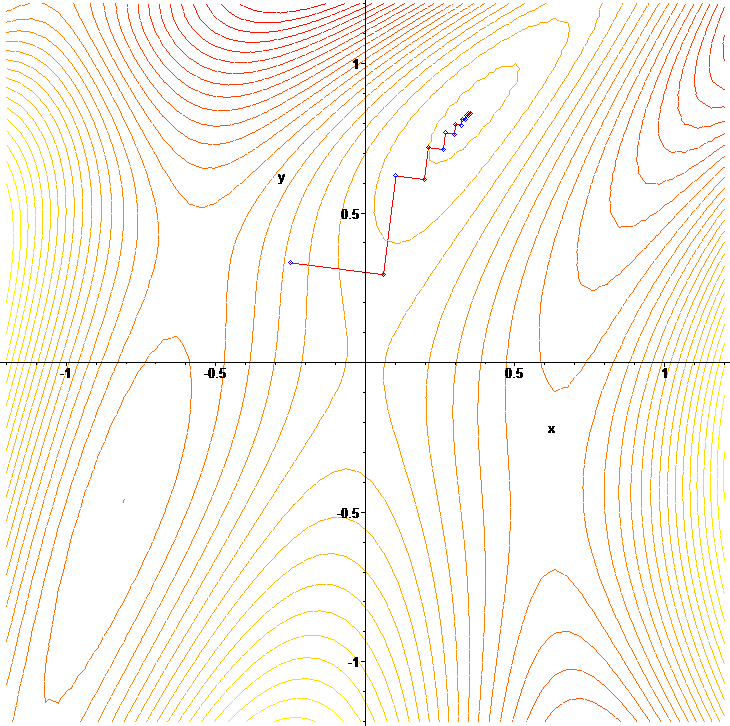
\includegraphics[width=0.45\textwidth]{images/gradient_ascent_contour.png}
  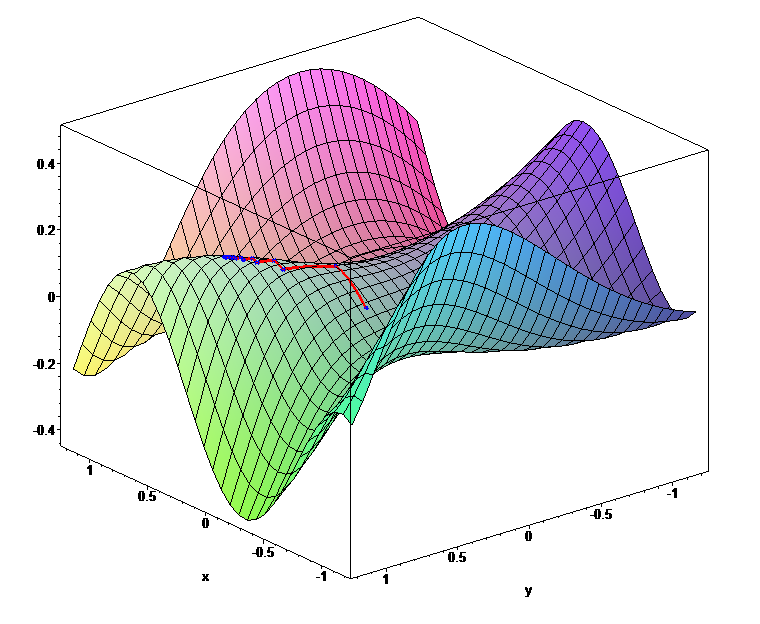
\includegraphics[width=0.45\textwidth]{images/gradient_ascent_surface.png}
  \caption{\label{fig:grad-desc}Visualización de la técnica de gradiente descendente, en este caso, buscando un máximo de la función $F(x,y)=\sin\left(\frac{1}{2} x^2 - \frac{1}{4} y^2 + 3 \right) \cos(2 x+1-e^y)$. Imágenes de Wikimedia Commons en dominio público}
\end{figure}

La técnica de gradiente descendente presenta algunos problemas: como se
puede observar en la \autoref{fig:grad-desc}, cuando el gradiente de
la función es próximo a cero el algoritmo tiende a dar pasos muy cortos,
convergiendo muy lentamente hacia el extremo local encontrado. Asimismo,
en general puede presentar un comportamiento de ``zig-zag'' para ciertas
funciones, avanzando de forma casi ortogonal al segmento que guarda la
distancia más corta con el extremo.
